\subsection{Architecture}
In het begin van de architectuur definieren we de benodigde signalen. Op basis van de hulpsignalen cnt en pwmi kunnen we een PWM signaal generen (zie verder). Daarna worden de nodige types en signalen aangemaakt om een \gls{fsm} te kunnen gebruiken. Eerst worden de verschillende staten gedefinieerd waarna de signalen voor het bijhouden van de staat (currentState en nextState) ook aangemaakt worden.

\lstinputlisting[firstline=1,lastline=14]{servocontroller_arch.vhd}
State\_trans beschrijft de transities tussen verschillende staten. De transities worden beschreven in volgend flowchart.
\begin{figure}[h]
	\centering
	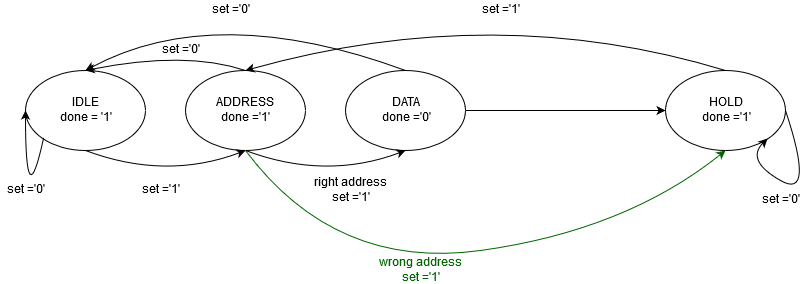
\includegraphics[width=\linewidth]{servocontrol.png}
	\caption{Transitiediagram voor de \gls{fsm} van de servocontroller}
\end{figure}\\
 Voordat de controller het \gls{pwm} signaal aanmaakt, moet er gecontroleerd worden of het doorgestuurde adres enerzijds het broadcast address is, of anderzijds het adres is van de servomotor is. Ander mag de controller zijn output niet aanpassen. Indien het set-signaal onderbroken wordt, voordat er een nieuwe positie is doorgestuurd, moet de controller naar de neutrale positie(idle) gaan.

\lstinputlisting[firstline=17,lastline=49]{servocontroller_arch.vhd}
Transition is het proces dat de overgangen van de staten dicteert. Hier wordt er ook voor gezorgd dat bij een reset de controller altijd terug gaat naar neutrale (idle) positie, ongeacht de status van de andere signalen.

\lstinputlisting[firstline=51,lastline=58]{servocontroller_arch.vhd}
Set\_output dicteert hoe het done signalen zich gedraagt in elke staat. In deze setup heeft done een tri-state logic. Het \gls{pwm} signaal wordt hier niet gedefinieerd omdat er een one-line process gebruikt wordt om dit aan de uitgang te koppelen (zie verder).

\lstinputlisting[firstline=60,lastline=82]{servocontroller_arch.vhd}
Pwm\_data is het proces dat de berekeningen en lengte van de puls bepaalt. Op basis van de servoklok wordt berekend welke waarden nodig zijn om de gewenste pulsen te bekomen. In de commentaar zijn de berekende waarden voor een servoklok van 510kHz te vinden. Indien de servoklok aangepast wordt, moet deze code aangepast worden zodat de juiste waarden gebruikt worden.

\lstinputlisting[firstline=84,lastline=99]{servocontroller_arch.vhd}
Gen\_pwm is het proces dat de eigenlijke puls genereert. Het aantal servoklok ticks wordt bijgehouden en vergeleken met de benodigde aantallen die in pwm\_data bepaald zijn. Cnt moet gereset worden bij elke klok tick (50 Hz).\\
Nadien wordt met een one-line process het pwm signaal aan de output gekoppeld.

\lstinputlisting[firstline=101,lastline=114]{servocontroller_arch.vhd}